\documentclass[12pt,letterpaper]{article}

\usepackage{ucs}
\usepackage[utf8x]{inputenc}
\usepackage[T1]{fontenc}
\usepackage{amsmath}
\usepackage{amsfonts}
\usepackage{amssymb}
\usepackage{graphicx}
\usepackage{fullpage}

\usepackage[colorlinks=true, 
            pdfstartview=FitV, 
            linkcolor=black, 
            citecolor=black,
            urlcolor=black]{hyperref}

\date{\today}
\author{Charles Varin}
\title{Optical response of a dipolar medium for integration with the finite-differences time-domain method for solving the Maxwell equations}

\begin{document}
\maketitle 
\tableofcontents
\section{Introduction}\label{intro}
In the presence of a medium with an electric susceptibility (but no free charges), the evolution of the electric and magnetic field vectors $\mathbf{E}$ and $\mathbf{H}$ is given by the following Maxwell equation:
\begin{subequations}\label{eq:maxwell}
  \begin{align}\label{eq:maxwell1}
   \frac{\partial\mathbf{E}}{\partial t} &=\frac{1}{\epsilon}\nabla\times\mathbf{H}-\frac{1}{\epsilon}\frac{\partial\mathbf{P}}{\partial t},\\
   \frac{\partial\mathbf{H}}{\partial t} &=-\frac{1}{\mu_0}\nabla\times\mathbf{E},\label{eq:maxwell2}
  \end{align}
\end{subequations}
where $c = 1/\sqrt{\epsilon\mu_0}$ with $\epsilon = \epsilon_0\epsilon_r$. In the next sections, a model for the temporal evolution of the polarization $\mathbf{P}$ of a dipolar medium is presented. For general details regarding to the finite-differences time-domain (FDTD) method for solving Eqs. \eqref{eq:maxwell}, see \cite{sullivan2000,taflove2005}.

\section{Static response of a dipolar medium}\label{static}
A dipolar medium is composed of molecules that possess a permanent dipole moment and whose polarizability is anisotropic. In a static electric field, initially disordered molecules will tend to align along the field lines leading to an average polarization. Models for the static response associated with the permanent dipole moment and the anisotropic susceptibility can be found in \cite{jackson1999,hook1991} and \cite{boyd2008}, respectively. We here put those two models together and see that the result is not the same as if they were treated as independent contributions. 

A molecule in a static electric field rotates to align along the electric field lines. The potential energy is given by the dot product of the polarization (permanent and induced) and the electric field \cite{bonin1997}:
\begin{align}\label{eq:potential}
U &= -\mathbf{p}\cdot\mathbf{E}\nonumber\\
&=-\mathbf{p}_0\cdot\mathbf{E} - \frac{1}{2}\mathbf{E}\cdot\mathbf{\boldsymbol\alpha}\cdot\mathbf{E}\nonumber\\
&= -p_0E\cos\theta-\left[\alpha_\bot + (\alpha_\parallel - \alpha_\bot)\cos^2\theta\right]E^2,
\end{align}
where Eq. (4.4.8) of \cite{boyd2008} we used. The molecular polarization is thus:
\begin{equation}\label{eq:single_pol}
 p = p_0\cos\theta+\left[\alpha_\bot + (\alpha_\parallel - \alpha_\bot)\cos^2\theta\right]E,
\end{equation}
where $\alpha_\bot$ and $\alpha_\parallel$ are the first-order molecular polarizability, perpendicular and parallel to $\mathbf{p}_0$, respectively.

For a collection of molecules, the total polarization is the average over all the molecules times the number of molecules per unit volume:
\begin{equation}\label{eq:total_pol}
 P=N<p>=N\left\lbrace p_0<\cos\theta>+\left[\alpha_\bot + (\alpha_\parallel - \alpha_\bot)<\cos^2\theta>\right]E\right\rbrace.
\end{equation}
At equilibrium, $<\cos\theta>$ and $<\cos^2\theta>$ are given by:
\begin{subequations}\label{eq:statistics}
 \begin{align}
  <\cos\theta>&=\frac{\int_0^\pi\cos\theta\exp(-U/k_BT)\sin\theta d\theta}{\int_0^\pi\exp(-U/k_BT)\sin\theta d\theta},\\
  <\cos^2\theta>&=\frac{\int_0^\pi\cos^2\theta\exp(-U/k_BT)\sin\theta d\theta}{\int_0^\pi\exp(-U/k_BT)\sin\theta d\theta},
 \end{align}
\end{subequations}
where $U$ is a function of $\theta$. 

Analytical solutions for Eqs.~\eqref{eq:total_pol} and \eqref{eq:statistics} for the case where the polarizability is zero ($\alpha_\bot = \alpha_\parallel=0$) can be found in \cite{hook1991} (Sec. 9.1.3) and \cite{jackson1999} (Sec. 4.6). The solution for $p_0 = 0$ can be found in \cite{boyd2008} (Sec. 4.4). The complete solution ($p_0\neq 0$, $\alpha_\bot\neq 0$, and $\alpha_\parallel\neq 0$) was found numerically and is compared with the analytical formulas in Fig. \ref{fig:stat_pol}.

\begin{figure}
    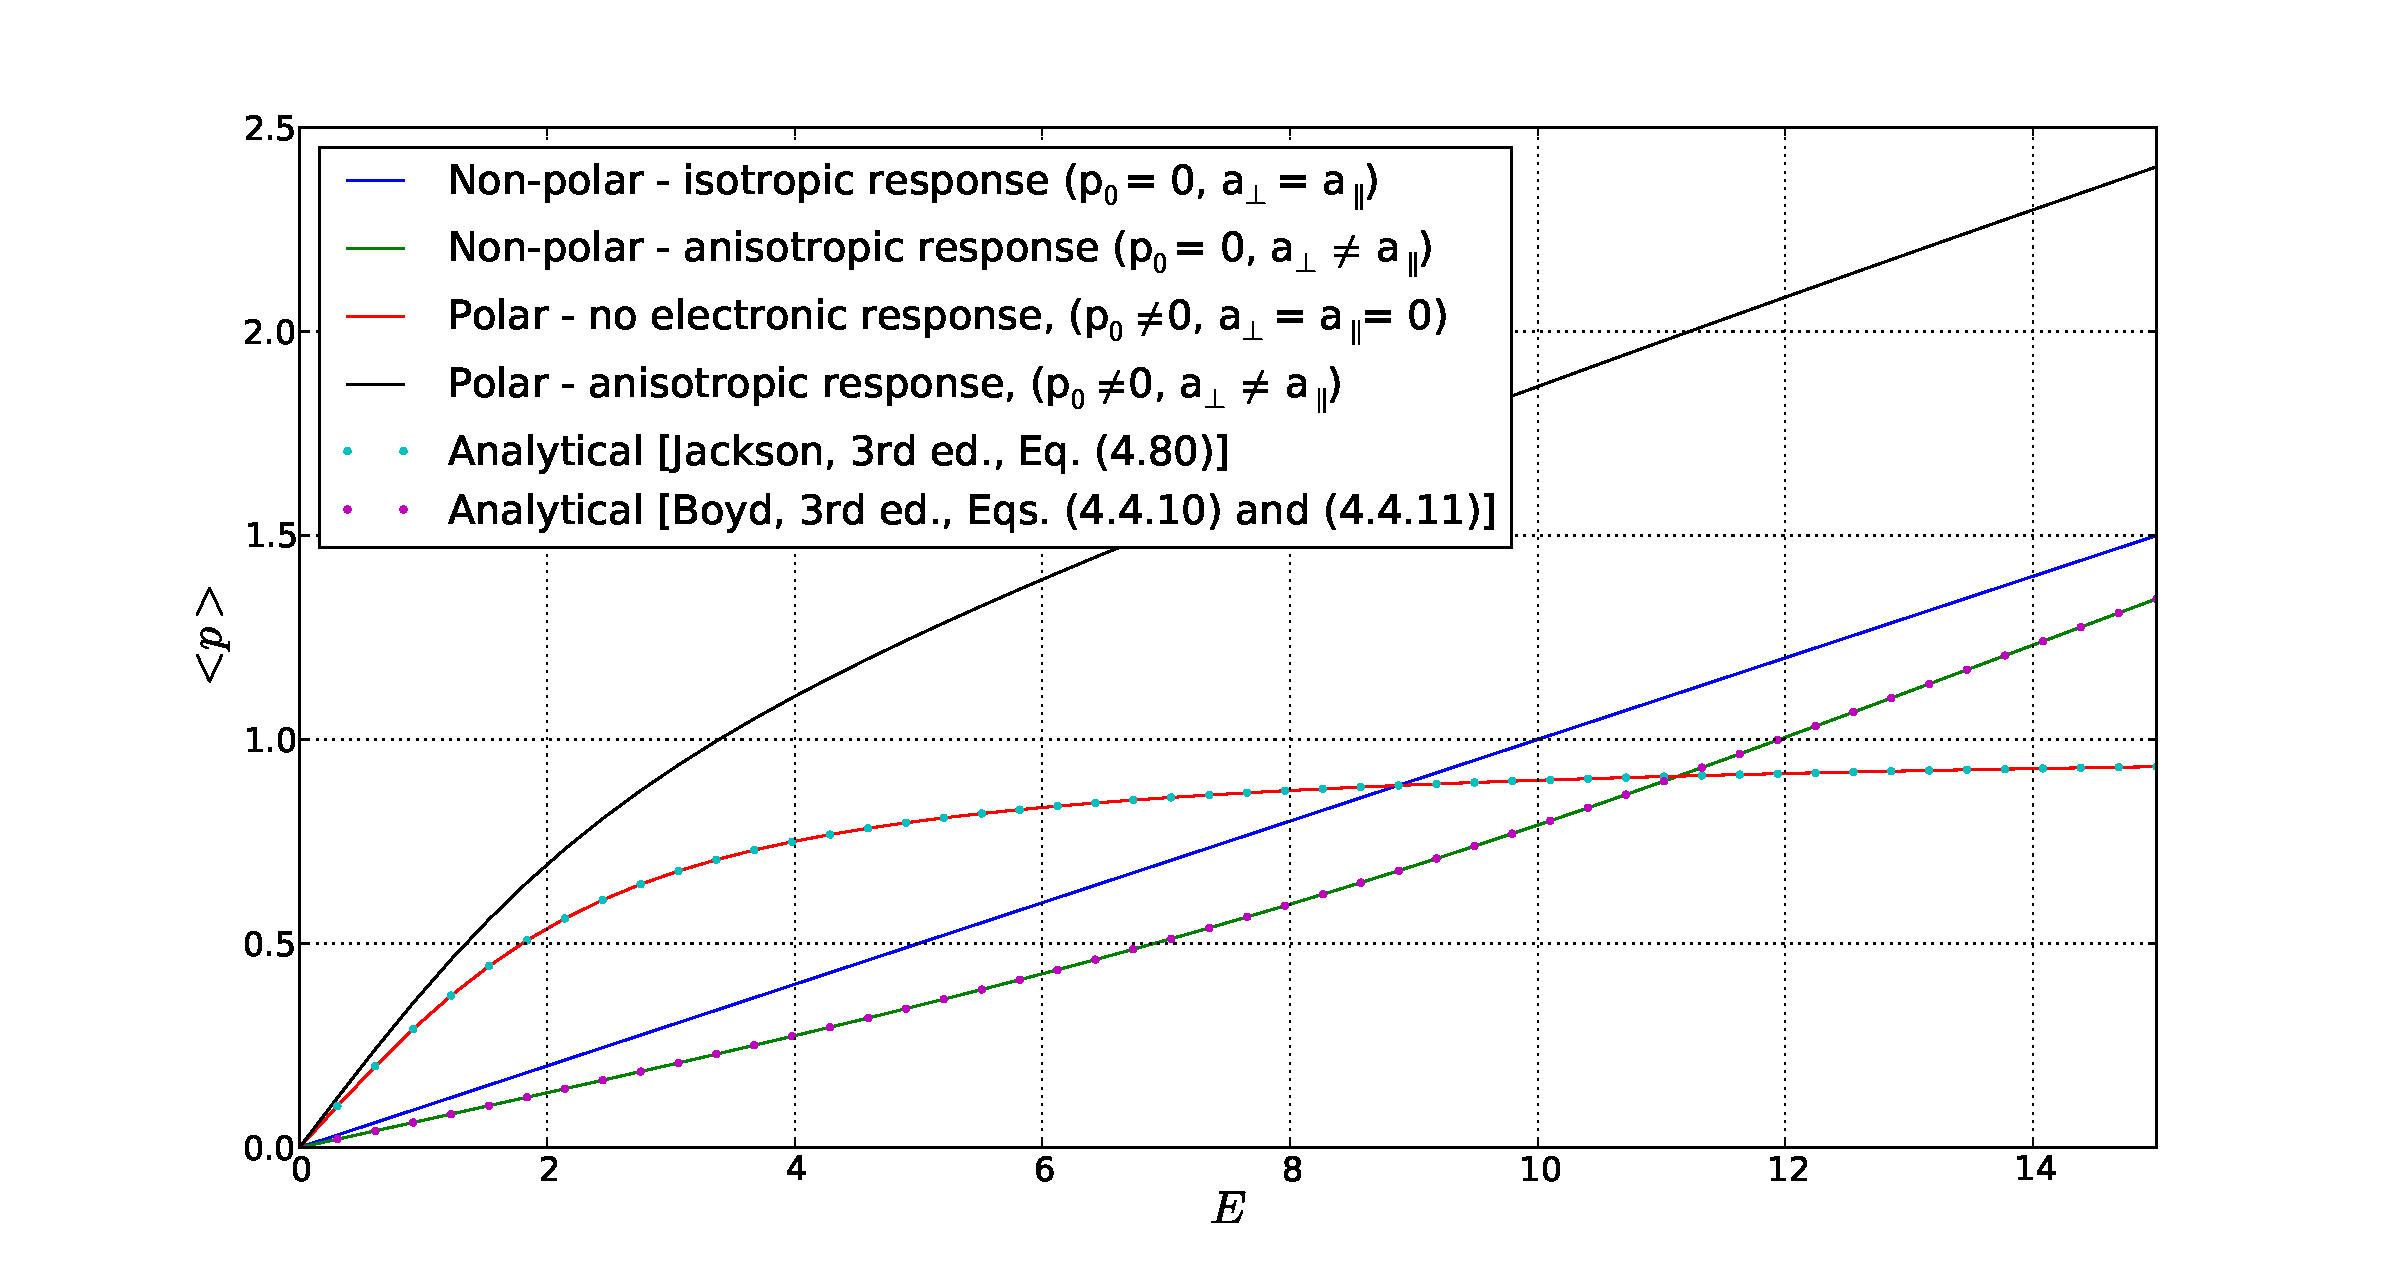
\includegraphics[width=17.2cm]{static_polarization.pdf}
    \caption{Average molecular polarization at equilibrium as a function of the electric field.}
    \label{fig:stat_pol}
\end{figure} 

For three-dimensional problems, the potential can be written as 
\begin{align}\label{eq:potential_altern}
U &= \sum_{i=x,y,z} p_0E_i\cos\theta_i+\left[\alpha_\bot + (\alpha_\parallel - \alpha_\bot)\cos^2\theta_i\right]E_i^2,
\end{align}
and each $<\cos\theta_i>$ and $<\cos^2\theta_i>$ can be calculated independently using Eqs. \eqref{eq:statistics}. The components of the polarization are then:
\begin{equation}\label{eq:pol_components}
 P_i=N<p_i>=N\left\lbrace p_0<\cos\theta_i>+\left[\alpha_\bot + (\alpha_\parallel - \alpha_\bot)<\cos^2\theta_i>\right]E_i\right\rbrace.
\end{equation}

\section{Weak-field polarizability}\label{weak_field}
Before going into the time evolution of the molecular polarization, we will define the material response in the limit where the field is weak, i.e., when $E\rightarrow 0$. In other words, we will find the linear response so that $<p>_0=<\alpha>_0 E$. For that, we expand the exponentials in Eqs. \eqref{eq:statistics}:
\begin{align}
  \exp(-U/k_BT)\simeq 1-\frac{U}{k_BT} = 1+\frac{p_0E\cos\theta+\left[\alpha_\bot + (\alpha_\parallel - \alpha_\bot)\cos^2\theta\right]E^2}{k_BT}.
\end{align}
The evaluation of the average values then gives:
\begin{subequations}\label{eq:statistics_weak_field}
 \begin{align}
  <\cos\theta>&=\frac{p_0 E}{3k_BT},\\
  <\cos^2\theta>&=\frac{1}{3}.
 \end{align}
\end{subequations}
and we find
\begin{equation}\label{eq:total_pol_weak_field}
 <p>_0=\left[\frac{p_0^2 }{3k_BT}+\left(\frac{1}{3}\alpha_\parallel + \frac{2}{3}\alpha_\bot\right)\right] E,
\end{equation}
in agreement with \cite{jackson1999,hook1991,boyd2008}. This can be converted to a linear refractive index ($n_0$), or linear relative electric permittivity ($\epsilon_r$).


\section{Time evolution of the molecular polarizability}\label{time}

\bibliographystyle{unsrt} 
\bibliography{dipmed}
\end{document}
